\documentclass[conference]{IEEEtran}
\usepackage[T1]{fontenc}
\usepackage[utf8]{inputenc}
\usepackage{cite}
\usepackage{amsmath,amssymb}
\usepackage{booktabs,tabularx,array}
\usepackage{graphicx}
\usepackage{xcolor}
\usepackage{listings}
\usepackage{tikz}
\usetikzlibrary{arrows.meta,positioning}
\usepackage[hidelinks]{hyperref}
\urlstyle{same}
\lstset{basicstyle=\ttfamily\scriptsize,breaklines=true,columns=fullflexible,
 keepspaces=true,showstringspaces=false,frame=single,captionpos=b}
\newcommand{\kg}[1]{\texttt{kg:#1}}
\newcommand{\code}[1]{\texttt{#1}}
\title{Linked Open Data Application\\for a Movie Knowledge Graph}
\author{
\IEEEauthorblockN{Do Tuan Hoang}
\IEEEauthorblockA{20261219M\\
\href{mailto:Hoang.DT261219M@sis.hust.edu.vn}{Hoang.DT261219M@sis.hust.edu.vn}}
\and
\IEEEauthorblockN{Nguyen Truong Huy}
\IEEEauthorblockA{20261260M\\
\href{mailto:Huy.NT261260M@sis.hust.edu.vn}{Huy.NT261260M@sis.hust.edu.vn}}
}
\begin{document}
\maketitle
\begin{abstract}
This project builds a movie knowledge graph from the TMDB 5000 dataset. We prepare eleven CSV tables, transform them into RDF, and define an OWL ontology for movies, people, acting roles, genres, countries, languages, and keywords. The graph uses our own vocabulary and stores ratings directly on movies. We also link local entities to Wikidata and DBpedia. SPARQL queries demonstrate movie search, filtering, and relationships inferred from the ontology. The current dataset contains 100 movies and 11,603 RDF triples. A Python command-line interface supports querying with or without reasoning.
\end{abstract}

\begin{IEEEkeywords}
Linked Data, movie knowledge graph, TMDB, RDF, OWL, SPARQL, entity linking
\end{IEEEkeywords}
\section{Introduction}
Movie datasets contain many relationships between films, actors, directors, genres, and countries. In CSV files, these relationships are often stored as nested lists or repeated values. A knowledge graph represents them explicitly as connections between resources. RDF provides the triple representation, while SPARQL allows us to query the connected data~\cite{w3c2014rdf11,w3c2013sparql}.

Our goal is to build a Linked Open Data application for the movie domain. We follow the workflow of the supplied Movie-Knowledge-Graph reference project: prepare data, transform it into RDF, define an ontology, establish external links, and query the graph. We adapt this workflow to the TMDB 5000 CSV dataset instead of collecting movies through the live API. We also remove production companies and vote counts, add keywords, and use a local vocabulary.

The following sections describe the method, data preparation, ontology, linking, and query results. The application currently runs through a command-line interface.

\section{Methodology}\label{sec:method}
The project follows five steps. First, we explore the raw movie and credit files and choose the information needed for our questions. Second, we split the data into CSV tables. Third, we define the ontology and transform the tables into RDF. Fourth, we link local entities to Wikidata and DBpedia. Finally, we query the graph using SPARQL, with reasoning enabled when needed.

Figure~\ref{fig:pipeline} summarizes the workflow. The ontology and movie data are stored separately. The query program combines them in memory, with external link files loaded when requested.

\begin{figure}[t]
\centering
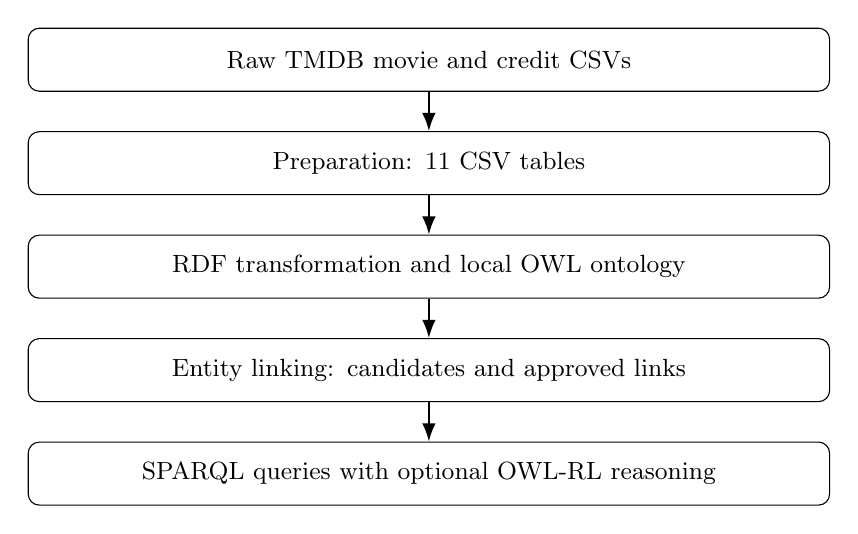
\begin{tikzpicture}[
 node distance=5mm,
 box/.style={draw,rounded corners,align=center,font=\small,
 text width=.82\columnwidth,minimum height=8mm},
 arr/.style={-{Latex},thick}]
\node[box] (raw) {Raw TMDB movie and credit CSVs};
\node[box,below=of raw] (prep) {Preparation: 11 CSV tables};
\node[box,below=of prep] (rdf) {RDF transformation and local OWL ontology};
\node[box,below=of rdf] (link) {Entity linking: candidates and approved links};
\node[box,below=of link] (query) {SPARQL queries with optional OWL-RL reasoning};
\draw[arr] (raw)--(prep);
\draw[arr] (prep)--(rdf);
\draw[arr] (rdf)--(link);
\draw[arr] (link)--(query);
\end{tikzpicture}
\caption{Overview of the project workflow. Local queries can also run before external linking.}
\label{fig:pipeline}
\end{figure}

\paragraph{Movie ontology}
We use the namespace \url{https://example.org/ontology/}, abbreviated as \code{kg:}. The ontology contains seven classes. Movie represents films; Person represents actors and directors; Role stores an acting credit; Genre, Country, Language, and Keyword describe related entities. Ratings are decimal values on Movie rather than separate resources.

\begin{table}[t]
\caption{Main vocabulary of our movie ontology.}
\centering\small
\begin{tabularx}{\columnwidth}{@{}lX@{}}
\toprule Category & Terms, using the kg: prefix\\\midrule
Classes & Movie, Person, Role, Genre, Country, Language, Keyword\\
Object properties & actor, director, directedMovie, hasCastMember, genre, keywords, countryOfOrigin, inLanguage, referencePage\\
Datatype properties & name, abstract, characterName, datePublished, duration, position, ratingValue\\
\bottomrule\end{tabularx}
\end{table}

\paragraph{Evaluation protocol}
Following the reference, we demonstrate basic retrieval, filtering and aggregation, reasoning-based queries, and external links. We run the queries on the generated RDF and compare selected results before and after reasoning. The results describe only our sample, not the complete TMDB catalogue.

The questions guide the model: cast questions require shared person identities,
character questions require acting-role nodes, and thematic search requires
movie-to-keyword relationships. We do not infer universal rules, such as exactly
one director per movie, from the small sample.

\section{Data collection and transformation}\label{sec:data}
\subsection{Data collection}
We use the movie and credit files from the TMDB 5000 dataset on Kaggle. The preparation script selects the first 100 distinct movies, keeps up to ten cast members per movie in credit order, and retains directors only from the crew. Movie and credit records are joined by movie ID.

Movie fields include title, overview, original language, release date, runtime, and average rating. Nested lists provide genres, countries, spoken languages, and keywords. We exclude companies, budget, revenue, and vote counts to keep the model small. The input does not provide IMDb IDs.

\begin{table}[t]
\caption{Prepared CSV tables.}
\centering\small
\begin{tabular}{lr}
\toprule Table & Rows\\\midrule
movies & 100\\
genres & 14\\
movie\_genres & 330\\
countries & 19\\
movie\_countries & 150\\
languages & 23\\
movie\_languages & 170\\
cast & 1,000\\
crew & 111\\
keywords & 667\\
movie\_keywords & 1,049\\
\bottomrule\end{tabular}
\end{table}

The script checks dates and numeric values, removes exact duplicate rows, and preserves missing values as empty cells. The eleven tables include reusable entity records and movie-to-entity relationships.

\subsection{Data transformation}
The transformer follows the reference's RDFLib implementation. Each identified entity receives a URI based on its type and source ID, such as \url{https://example.org/movie/558}. A person keeps the same URI across acting and directing credits.

Titles and descriptions become literals. Release dates use \code{xsd:date}, runtime uses \code{xsd:duration}, and average rating uses \code{xsd:decimal}. Missing values are omitted. Original and spoken languages share \kg{inLanguage}. Movie production countries remain available even though companies are excluded.

Acting credits use both a direct movie--person relationship and a Role blank node when character or cast-order information is available. The role holds details specific to that film:
\begin{lstlisting}
ex:film kg:actor ex:person, [
  a kg:Role ;
  kg:actor ex:person ;
  kg:characterName "Pilot" ;
  kg:position 0
] .
\end{lstlisting}
Here, \code{ex:} represents example resources. The output file, \path{output/movies.ttl}, contains 11,603 triples for the current sample.

\begin{table}[t]
\caption{Examples of the CSV-to-RDF mapping.}
\label{tab:mapping}
\centering\small
\begin{tabularx}{\columnwidth}{@{}lX@{}}
\toprule Source field & RDF representation\\\midrule
Movie ID & Part of the movie URI, not its display title\\
Title & \kg{name}, string literal\\
Release date & \kg{datePublished}, \code{xsd:date}\\
Runtime & \kg{duration}, e.g., \code{PT120M}\\
Vote average & \kg{ratingValue}, \code{xsd:decimal}\\
Keyword ID & Shared Keyword resource via \kg{keywords}\\
Character and order & \kg{characterName} and \kg{position} on Role\\
\bottomrule
\end{tabularx}
\end{table}

Table~\ref{tab:mapping} shows how source values become either resource identifiers,
relationships, or literals. Titles are used for display and search; IDs preserve
identity even when different movies have the same title. A character name is
attached to a role because a person can play different characters in different
movies. Ratings need only one literal in our model, so no separate rating node
is created.

\section{Ontology construction and entity linking}\label{sec:onto}
\subsection{Ontology construction}
Figure~\ref{fig:owl-design} shows our OWL ontology design, summarizing the main movie-domain classes and their relationships.
\begin{figure}[htbp]
\centering
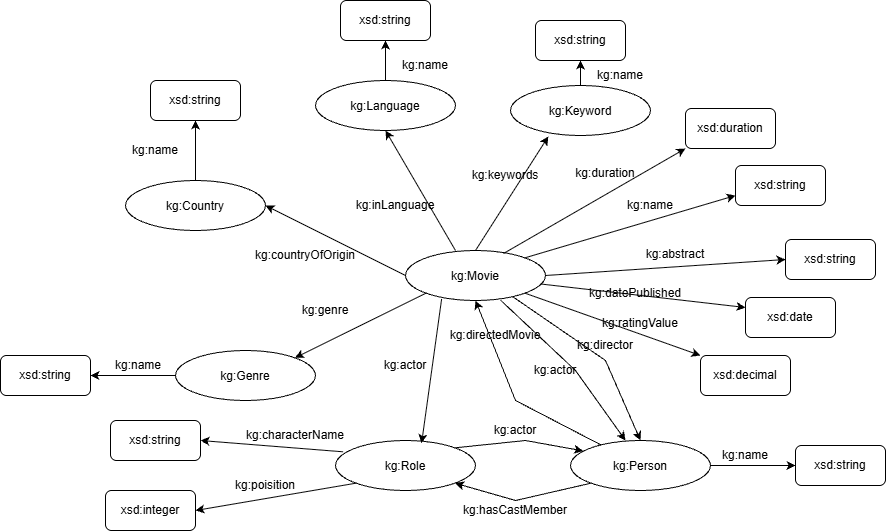
\includegraphics[width=\linewidth,keepaspectratio]{images/ontology.png}
\caption{OWL ontology design for the movie knowledge graph.}
\label{fig:owl-design}
\end{figure}

The ontology defines classes, property domains and ranges, disjoint classes, and cardinality restrictions. Our domain terms use \code{kg:} instead of Schema.org. We do not include broad superclasses such as CreativeWork or Thing.

A movie has at least one name and at most one rating value. An acting role has exactly one actor of type Person, at most one character name, and at most one cast position. These OWL restrictions describe the intended model; missing fields still need separate checks because OWL uses an open-world interpretation.

Two axioms support our reasoning examples. First, \kg{directedMovie} is the inverse of \kg{director}. Second, the path from a director to a directed movie and then to its actors implies \kg{hasCastMember}:
\begin{lstlisting}
kg:directedMovie
  owl:inverseOf kg:director .

kg:hasCastMember
  owl:propertyChainAxiom
    (kg:directedMovie kg:actor) .
\end{lstlisting}
Because actor can point to a person or an acting role, hasCastMember can also point to either. Queries listing actors explicitly select Person resources.


% Figure~\ref{fig:reasoning} illustrates the property chain with example resources.
% The directedMovie edge can first be inferred from a movie's director edge.
% Following it with an actor edge then produces hasCastMember.

% \begin{figure}[t]
% \centering
% \begin{tikzpicture}[
%  n/.style={draw,rounded corners,font=\small,minimum height=7mm},
%  edge/.style={-{Latex},thick},
%  lab/.style={font=\scriptsize,fill=white,inner sep=2pt}]
% \node[n] (director) at (0,0) {Director};
% \node[n] (movie) at (2.3,0) {Movie};
% \node[n] (actor) at (4.6,0) {Actor};
% \draw[edge] (director)--node[lab,above]{directedMovie}(movie);
% \draw[edge] (movie)--node[lab,above]{actor}(actor);
% \draw[edge,dashed] (director.south) to[bend right=35]
%  node[lab,below]{hasCastMember (inferred)} (actor.south);
% \end{tikzpicture}
% \caption{A director-to-actor relationship derived through a movie. Property names use the kg: prefix.}
% \label{fig:reasoning}
% \end{figure}

\subsection{Entity linking}
Movies are matched to Wikidata using their TMDB movie IDs and release years. A matching ID and year allow automatic approval. Weaker candidates require review, while conflicting years can cause rejection. Title matching is used as a fallback. People are matched using TMDB person IDs, human type, and normalized names. Name and filmography searches provide fallback candidates.

Countries and languages are matched by ISO codes. Genres are matched using film-genre names and linked with \code{skos:closeMatch}, since the genre categories may not have exactly the same meaning. Movies, people, countries, and languages use \code{owl:sameAs} for approved identity matches.

The scripts save candidate evidence in CSV files and approved links in separate Turtle files. The current outputs contain 198 movie links, 1,591 person links, and 112 lookup links. DBpedia URIs are constructed from English Wikipedia titles returned by Wikidata; they have not been independently checked against DBpedia. Automatic approval therefore does not guarantee that every link is correct.

\section{Evaluation}\label{sec:eval}
We evaluate the graph using the same types of questions as the reference project. The following results come from our current local dataset.

\subsection{Basic retrieval}
A simple query checks whether the sample contains Spider-Man movies:
\begin{lstlisting}
PREFIX kg: <https://example.org/ontology/>
SELECT ?title WHERE {
  ?movie a kg:Movie ; kg:name ?title .
  FILTER(CONTAINS(LCASE(STR(?title)), "spider"))
}
ORDER BY ?title
\end{lstlisting}
It returns four titles: Spider-Man 2, Spider-Man 3, The Amazing Spider-Man, and The Amazing Spider-Man 2.

\subsection{Structured filtering and aggregation}
The rating query selects Drama movies and orders them by average rating. Unlike the reference, it reads the rating directly from Movie:
\begin{lstlisting}
PREFIX kg: <https://example.org/ontology/>
SELECT ?title ?rating WHERE {
  ?movie a kg:Movie ; kg:name ?title ;
    kg:genre ?genre ; kg:ratingValue ?rating .
  ?genre kg:name "Drama" .
}
ORDER BY DESC(?rating) ?title
LIMIT 20
\end{lstlisting}
The query returns fifteen films. Table~\ref{tab:rating} shows the first three. Other queries count repeated actor collaborations and find directors with multiple films.
\begin{table}[h]
\caption{First three results of the Drama rating query.}
\label{tab:rating}\centering\small
\begin{tabular}{lr}
\toprule Movie & Rating\\\midrule
The Dark Knight & 8.2\\
Interstellar & 8.1\\
Inside Out & 8.0\\
\bottomrule\end{tabular}
\end{table}

\subsection{Reasoning-based queries}
Query 11 asks for a person's directed movies using \kg{directedMovie}. It returns no results before reasoning because the transformer stores \kg{director} instead. With OWL-RL reasoning, the inverse relationship is inferred and the query returns twenty rows, its specified limit.

Query 12 uses \kg{hasCastMember} to find actors in movies directed by a person. It returns no rows before reasoning and 1,023 rows after reasoning, without external links loaded. This query has no result limit in the current version. These examples show the effect of the inverse and property-chain axioms.


\begin{table}[t]
\caption{Effect of reasoning on the two inference queries, without external links.}
\label{tab:inference-results}
\centering\small
\begin{tabularx}{\columnwidth}{@{}Xrr@{}}
\toprule Query & Before & After\\\midrule
Q11: directed movies & 0 & 20\\
Q12: director--actor pairs & 0 & 1,023\\
\bottomrule
\end{tabularx}
\end{table}

Table~\ref{tab:inference-results} compares the same queries on asserted data and
after loading the ontology and applying reasoning. Q11 is limited to twenty
results; Q12 has no limit. The additional answers follow from local facts and
ontology axioms, rather than new information downloaded from the Web.

\subsection{Cross-knowledge-graph queries}
We can list the external links associated with each movie:
\begin{lstlisting}
PREFIX kg: <https://example.org/ontology/>
PREFIX owl: <http://www.w3.org/2002/07/owl#>
SELECT ?title ?external WHERE {
  ?movie a kg:Movie ; kg:name ?title ;
    owl:sameAs ?external .
}
\end{lstlisting}
This query reads the stored links; it does not download external facts. A separate SERVICE query is available for requesting Wikidata information, but remote results were not evaluated here. Its example movie ID must be changed to a linked movie from our sample.

\subsection{SPARQL command-line interface}
Our implementation uses \path{scripts/ask.py} instead of a deployed Fuseki endpoint. The script loads the movie data, ontology, and any specified link files into one RDFLib graph. The \code{--reasoning} option applies OWL-RL before running the query.

All 32 existing unit tests passed. After reasoning with all link files, the missing-name and disjoint-type checks returned no rows. These checks cover specific problems and do not prove complete ontology correctness.

\section{Discussion}\label{sec:discussion}
The graph supports movie search, rating queries, shared-person relationships, and inferred director-to-cast relationships. Our smaller model keeps these functions while replacing companies with keywords and simplifying ratings.

\paragraph{Limitations}
The dataset contains only 100 movies and the first ten cast members per movie. It cannot describe every collaboration. Without vote counts, ratings cannot be filtered by the number of voters. Original and spoken languages are combined. External matches can be uncertain, and DBpedia targets still need verification. Loading identity links does not retrieve remote facts; reasoning may also return multiple equivalent URIs for one entity.

\paragraph{Future work}
We can review uncertain links, verify DBpedia resources, and test remote queries. A Fuseki endpoint could provide browser-based SPARQL access. For public five-star Linked Open Data, the development URIs must also be replaced by persistent public identifiers and the data made available under suitable publication terms~\cite{bernerslee2006linkeddata}.

\section{Conclusion}\label{sec:conclusion}
We built a movie knowledge graph from the TMDB 5000 dataset using CSV preparation, RDF transformation, a local OWL ontology, and external entity links. The application follows the reference project's workflow with a smaller model: no companies or vote counts, direct movie ratings, and added keywords. SPARQL examples demonstrate retrieval, filtering, and reasoning through the command-line interface. Further work will focus on link verification, remote querying, and public deployment.

\bibliographystyle{IEEEtran}
\bibliography{references}
\appendices
\section{Running the application}
Run the following commands from the \code{semantic-web} directory after installing \path{requirements.txt}:
\begin{lstlisting}
python scripts/prepare.py
python scripts/transform.py
python scripts/ask.py -q queries/4.sparql
python scripts/ask.py -q queries/11.sparql --reasoning
python scripts/ask.py -q queries/show_links.sparql --links output/movie_links.ttl
\end{lstlisting}
The final two commands illustrate reasoning and loading a link file. Additional link files can be supplied by repeating \code{--links}. The original files are not changed by querying.

\end{document}
